\documentclass[main.tex]{subfiles}
\usepackage[utf8]{inputenc}
\usepackage[
backend=biber,
style=alphabetic,
sorting=ynt
]{biblatex}
\usepackage{subfiles}

\addbibresource{../references.bib} %Imports bibliography file

% Document information
\title{Proceso}
\author{Rocío Mena}
\date{\today}

\begin{document}

\maketitle

\subsection{Estrategia de Validación}

Implementar el modelo en V para el desarrollo de este trabajo implica seguir un enfoque estructurado y sistemático para las pruebas, que puede abarcar distintos tipos de pruebas, desde pruebas unitarias en cada módulo hasta pruebas de integración, sistema y aceptación. Este enfoque sistémico garantiza que el sistema cumpla con los requisitos técnicos y de negocio, y que sea robusto, seguro y eficiente desde su primera entrega.

Una estrategia de validación en software se refiere al conjunto de actividades planificadas para asegurar que un sistema o producto cumpla con los requisitos esperados y funcione correctamente bajo diferentes escenarios. Esta estrategia proporciona una guía detallada que describe los pasos a seguir durante las pruebas, define cuándo deben realizarse y estima el esfuerzo, tiempo y recursos necesarios para su implementación. La importancia de una estrategia de validación radica en su capacidad para estructurar el proceso de pruebas, evitando así esfuerzos innecesarios, errores no detectados y asegurando la calidad del software \cite{pressman2010ingeneria}

Para garantizar la eficacia de las pruebas, una estrategia de validación debe incluir varios elementos clave, tales como la planificación de pruebas, el diseño de casos de prueba, la ejecución de pruebas y la evaluación de los resultados obtenidos. Este proceso no solo asegura que el software funcione según lo previsto, sino que también permite identificar errores cometidos durante las fases de diseño y desarrollo, mejorando la calidad final del producto.

En el caso del desarrollo basado en el modelo en V, las pruebas se realizan de manera estructurada desde las pruebas de módulos individuales hasta las pruebas de integración, sistema y aceptación. Este enfoque sistemático asegura que el sistema funcione correctamente tanto a nivel de componentes como en su conjunto, permitiendo que el cliente y los usuarios finales participen en la validación y aceptación del sistema antes de su implementación.

\begin{figure}[h]
	\centering
	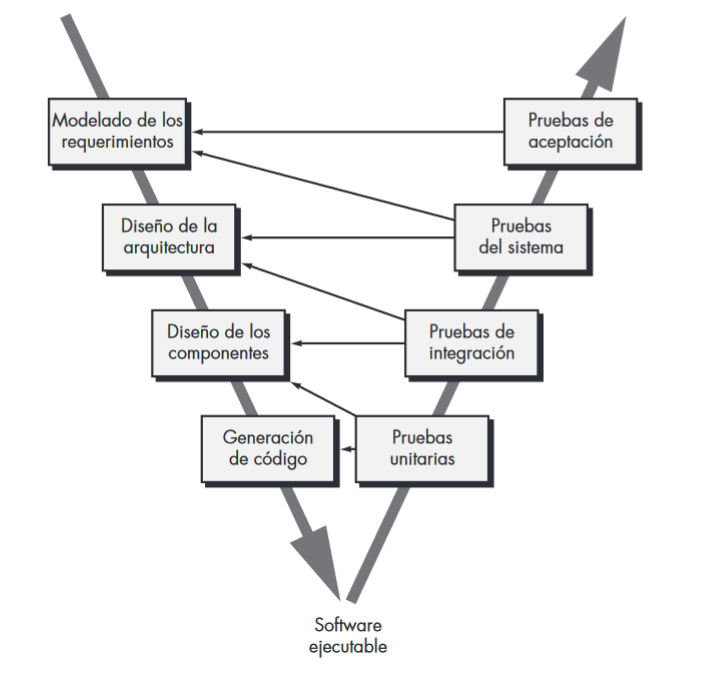
\includegraphics[width=\linewidth]{../assets/model-v.png}
	\caption{Modelo en V. Fuente: \cite{pressman2010ingeneria}}
\end{figure}

El desarrollo de una estrategia de validación eficaz permite evitar errores que podrían pasar desapercibidos en un enfoque de pruebas sin planificación. La validación sistemática permite una medición clara del progreso y asegura que cualquier problema emergente se detecte lo antes posible, optimizando el uso de tiempo y recursos. Al implementar este enfoque, se logra que el sistema sea estable, cumpla con los requerimientos y se entregue en tiempo y forma.

Para cada tipo de pruebas, es habitual definir un plan de pruebas, una lista de casos de prueba y un informe de resultados. Para los distintos tipos de prueba pueden utilizarse todos o sólo algunos de estos documentos, dependiendo del tipo de prueba, su granularidad y su criticidad.

\subsubsection{Pruebas Unitarias}

Las pruebas unitarias son pruebas que se aplican a los componentes más pequeños de un sistema, como componentes o métodos individuales. Su objetivo es verificar que cada unidad de código funcione correctamente en aislamiento.

Las pruebas unitarias por lo general se consideran como adjuntas al paso de codificación. El diseño de las pruebas unitarias puede ocurrir antes de comenzar la codificación o después de generar el código fuente. La revisión de la información del diseño proporciona una guía para establecer casos de prueba que es probable que descubran errores en cada una de las categorías analizadas anteriormente. Cada caso de prueba debe acoplarse con un conjunto de resultados esperados \cite{pressman2010ingeneria}.

Cada módulo de la arquitectura del sistema se desarrollará y validará de forma independiente antes de integrarse con otros módulos. Estas pruebas se centrarán en la funcionalidad individual de los módulos dentro cada uno de los componentes del sistema, asegurando que cada uno cumpla con los requisitos y expectativas definidos.

Para las pruebas unitarias se utilizan frameworks específicos para cada tecnología y lenguaje de programación. A su vez, estas pruebas se realizan con datos de prueba que cubran diferentes escenarios y casos límite, asegurando que el módulo funcione correctamente en todas las situaciones posibles, tanto normales como excepcionales.

La métrica habitual para evaluar la calidad de las pruebas unitarias es la cobertura de código, que mide el porcentaje de líneas de código que son ejecutadas por las pruebas. Una alta cobertura de código indica que las pruebas unitarias han validado la mayoría de las rutas de ejecución del código, lo que aumenta la confianza en la calidad del software. De todas formas, una alta cobertura de código no garantiza la ausencia de errores, motivo por el cual las pruebas unitarias son utilizadas junto con otros enfoques de pruebas para obtener una validación completa del sistema.

En nuestro trabajo, las pruebas unitarias tendrán el siguiente alcance:

\begin{itemize}
	\item \textbf{Plan de Pruebas Unitarias}: No se realizará un plan de pruebas unitarias formal, ya que estas pruebas se realizarán de forma continua durante el desarrollo de cada módulo. Sin embargo, para cada módulo del sistema se definirá el framework de pruebas a utilizar y el nivel de covertura mínimo requerido por las pruebas unitarias.
	\item \textbf{Casos de Prueba Unitarios}: No se realizará un documento formal de casos de prueba unitarios, debido a la alta granularidad de las pruebas unitarias. Estos casos se definirán y ejecutarán de forma continua durante el desarrollo de cada módulo. Durante el desarrollo se de definirán tantos casos de prueba como sea necesario para cubrir diferentes escenarios y casos límite para alcanzar el nivel de cobertura requerido.
	\item \textbf{Informe de Resultados}: No se realizará un informe formal de resultados de pruebas unitarias, ya que los resultados de las pruebas se documentarán directamente en el código fuente y en el sistema de control de versiones. Los resultados de las pruebas unitarias se pueden utilizar como informe de resultados en todo momento para evaluar el progreso y la calidad del desarrollo.
\end{itemize}

A continuación, como parte del plan de pruebas, se detallan los frameworks de pruebas unitarias a utilizar para cada tecnología y lenguaje de programación involucrados en el desarrollo del sistema. A su vez se detalla el nivel de covertura mínimo requerido por las pruebas unitarias para cada módulo del sistema.

\subsubsubsection{Aplicación Frontend}

\textbf{Framework}: para las pruebas unitarias del frontend del sistema se utilizará el framework Jest\footnote{https://jestjs.io} en conjunto con React Testing Library\footnote{https://testing-library.com/docs/react-testing-library/intro}. Estas dos herramientas suelen utilizarse en conjunto para realizar pruebas unitarias en aplicaciones Next.js y es la recomendación de la documentación oficial de Next.js para realizar pruebas en aplicaciones desarrolladas con este framework\footnote{https://nextjs.org/docs/app/building-your-application/testing/jest}. Jest es un framework de pruebas para JavaScript que permite escribir pruebas con una API accesible, familiar y rica en funcionalidades que proporciona resultados rápidamente. Jest está bien documentado, requiere poca configuración y puede extenderse para adaptarse a las necesidades del proyecto, a su vez, los repositorios Next.js ya proveen la configuración básica para este framework. React Testing Library es una biblioteca de pruebas específica para React que permite escribir pruebas que se centran en el comportamiento del usuario, en lugar de en la implementación interna de los componentes. Esta biblioteca fomenta las mejores prácticas de accesibilidad y proporciona una API sencilla y eficaz para escribir pruebas de componentes React.

\textbf{Cobertura Mínima}: se requerirá una cobertura mínima del 60\% para las pruebas unitarias del frontend del sistema. Este valor se considera adecuado para garantizar que la mayoría de las rutas de ejecución del código estén cubiertas por las pruebas unitarias. A su vez, el frontend de este prototipo es relativamente simple y no es una parte crítica del sistema, sino que se implementará con fines de demostración y validación de la funcionalidad del sistema, por lo que este valor de cobertura es suficiente para garantizar la calidad del código, sin requerir un esfuerzo excesivo en la escritura de pruebas unitarias.

\subsubsubsection{API de Trazabilidad}

\textbf{Framework}: para las pruebas unitarias de la API de trazabilidad se utilizará el framework Jest, que está integrado por defecto en el framework Nest.js y es el recomendado por la documentación oficial de Nest.js para realizar pruebas unitarias en aplicaciones desarrolladas con este framework\footnote{https://docs.nestjs.com/fundamentals/testing}.

\textbf{Cobertura Mínima}: se requerirá una cobertura mínima del 80\% para las pruebas unitarias de la API de trazabilidad. Dado que la API de trazabilidad es una parte crítica del sistema y es responsable de la comunicación con la blockchain y la base de datos SQL, es fundamental garantizar que todas las rutas de ejecución del código estén cubiertas por las pruebas unitarias. Un valor de cobertura del 80\% es adecuado para garantizar la calidad del código y minimizar el riesgo de errores en la implementación de la API. Este valor suele utilizarse en la industria como un estándar aceptable para la cobertura de código en aplicaciones críticas.

\subsubsubsection{Contratos Inteligentes}

\textbf{Framework}: para las pruebas unitarias de los contratos inteligentes se utilizará el framework Hardhat, que es uno de los frameworks de pruebas más utilizados en la industria para contratos inteligentes en Solidity. Hardhat proporciona un entorno de desarrollo completo para Ethereum, que incluye herramientas para compilar, desplegar y probar contratos inteligentes, así como para simular un entorno de blockchain local para pruebas unitarias\footnote{https://hardhat.org/hardhat-runner/docs/guides/test-contracts}. Dado que este framework se utilzará para el desarrollo de los contratos inteligentes, también se utilizará para las pruebas unitarias de los mismos.

\textbf{Cobertura Mínima}: se requerirá una cobertura mínima del 100\% para las pruebas unitarias de los contratos inteligentes. Dado que los contratos inteligentes son la base del sistema de trazabilidad, son responsables de la ejecución de las transacciones en la blockchain y teniendo en cuenta que una vez desplegados ya no pueden actualizarse, es fundamental garantizar que todos los caminos de ejecución del código estén cubiertos por las pruebas unitarias. Un valor de cobertura del 100\% es necesario para garantizar la calidad y la seguridad de los contratos inteligentes, minimizando el riesgo de errores en la implementación de los mismos. Este valor es un estándar en la industria para la cobertura de código en contratos inteligentes críticos.

\subsection{Pruebas de Integración}

Una vez que los módulos individuales han sido validados, el siguiente paso es probar la integración entre ellos dentro de cada capa y entre las diferentes capas. Las pruebas de integración son una técnica sistemática para construir la arquitectura del software mientras se llevan a cabo pruebas para descubrir errores asociados con la interfaz. El objetivo es tomar los componentes probados de manera individual y construir una estructura de
programa que se haya dictado por diseño \cite{pressman2010ingeneria}.

Las pruebas de integración se realizan para verificar que los módulos individuales funcionen correctamente juntos, pasando datos y ejecutando operaciones de manera fluida y sin errores. Estas pruebas se realizan siguiendo escenarios de uso que reflejen operaciones típicas y atípicas dentro del sistema, utilizando datos de prueba que simulen el entorno operativo real tanto como sea posible.

El método en V, por su estructura, propicia el uso de pruebas de integración ascendentes, que comienzan la construcción y la prueba con módulos atómicos (es decir, componentes en los niveles inferiores dentro de la estructura del programa). Puesto que los componentes se integran de abajo hacia arriba, la funcionalidad que proporcionan los componentes subordinados en determinado nivel siempre está disponible y se elimina la necesidad de representaciones intermedias \cite{pressman2010ingeneria}.

Las pruebas de integración en este sistema se realizarán con el objetivo de validar que las interfaces entre los módulos y las capas del sistema funcionen correctamente y que los datos se transmitan de manera adecuada entre ellos. Estas pruebas se centrarán en asegurar que la interfaz de usuario pueda comunicarse eficazmente con la API de trazabilidad y que esta, a su vez, interactúe correctamente con la blockchain y la base de datos SQL. 

Para las pruebas de integración se utilizarán datos de prueba que cubran diferentes escenarios y casos límite, asegurando que el sistema funcione correctamente en todas las situaciones posibles, tanto normales como excepcionales. Estas pruebas se realizarán en un entorno de desarrollo de pruebas controlado, simulando el entorno operativo real tanto como sea posible.

En nuestro trabajo, las pruebas de integración tendrán el siguiente alcance:

\begin{itemize}
	\item \textbf{Plan de Pruebas de Integración}: Estas pruebas se realizarán de forma manual y el plan de pruebas de integración únicamente listará los casos de uso a probar.
	\item \textbf{Casos de Prueba de Integración}: Se definirán casos de prueba de integración detallados para cada escenario de uso identificado en el plan de pruebas. Se utilizarán para guiar la ejecución de las pruebas de integración y para documentar los resultados obtenidos. Cada caso de prueba incluirá una descripción del escenario de uso, los datos de prueba a utilizar, los pasos a seguir y los resultados esperados.
	\item \textbf{Informe de Resultados de Integración}: Se generará un informe formal de resultados de pruebas de integración que documente los resultados obtenidos, los problemas identificados y las acciones correctivas tomadas. Este informe se utilizará para realizar ajustes y mejoras necesarias antes de las siguientes etapas de desarrollo y pruebas.
\end{itemize}

\subsection{Pruebas de Sistema}

Las pruebas de sistema consisten en una serie de diferentes pruebas cuyo propósito principal es ejercitar por completo el sistema implementado. Estas pruebas evalúan la calidad del sistema en su conjunto y comprueban su rendimiento bajo condiciones reales o simuladas. Aunque cada prueba tenga un propósito diferente, todo el conjunto de pruebas busca verificar que los elementos del sistema se hayan integrado de manera adecuada y que realicen las funciones asignadas. En estas pruebas se evalúan aspectos del sistema como la usabilidad, la confiabilidad, el rendimiento y la seguridad del sistema \cite{pressman2010ingeneria}.

Las pruebas de sistema se realizan en un entorno de pruebas controlado que simula el entorno operativo real del sistema, utilizando datos de prueba que reflejen situaciones reales y escenarios de uso típicos y atípicos. Algunas de estas pruebas se centran en validar que el sistema cumpla específicamente con los requerimientos no funcionales definidos en la etapa de análisis y diseño del sistema, y que sea capaz de realizar las funciones esperadas.

En nuestro trabajo, las pruebas de sistema tendrán el siguiente alcance:

\begin{itemize}
	\item \textbf{Plan de Pruebas de Sistema}: Se definirá un plan de pruebas de sistema que describa los escenarios de uso a probar, los criterios de aceptación y los datos de prueba a utilizar. Este plan de pruebas se utilizará como guía para la ejecución de las pruebas de sistema y para documentar los resultados obtenidos.
	\item \textbf{Casos de Prueba de Sistema}: Se definirán casos de prueba de sistema detallados para cada escenario de uso identificado en el plan de pruebas. Estos casos de prueba se utilizarán para guiar la ejecución de las pruebas de sistema y para documentar los resultados obtenidos. Cada caso de prueba incluirá una descripción del escenario de uso, los datos de prueba a utilizar y los resultados esperados.
	\item \textbf{Informe de Resultados de Sistema}: Se generará un informe formal de resultados de pruebas de sistema que documente los resultados obtenidos, los problemas identificados y las acciones correctivas tomadas. Este informe se utilizará para realizar ajustes y mejoras necesarias antes de la entrega final del sistema.
\end{itemize}

\subsection{Pruebas de Aceptación}

Las pruebas de aceptación, por otro lado, son pruebas realizadas por el cliente o el usuario final para determinar si el sistema cumple con los criterios de aceptación definidos previamente al comienzo del proyecto y durante su desarrollo. Estas pruebas se realizan en un entorno de pruebas controlado y se centran en validar que el sistema cumpla con los requisitos del negocio y las expectativas del usuario. Las pruebas de aceptación son esenciales para garantizar que el sistema sea aceptado por el cliente y los usuarios finales y que cumpla con sus necesidades y expectativas.

Debido al alcance de este trabajo académico, no se realizarán pruebas de aceptación formales con el cliente o los usuarios finales. Sin embargo, se realizarán pruebas de aceptación internas junto con las pruebas de sistema para validar que el sistema cumpla con los criterios de aceptación definidos en la etapa de análisis y diseño del sistema. Estas pruebas se realizarán de forma manual en un entorno de pruebas controlado y se centrarán en validar que el sistema cumpla con los requerimientos funcionales del sistema definidos en la etapa de análisis y diseño.

\end{document}
